\subsection{Topological Data Analysis}
\label{sec:si_tda}
Since the exact manifold (or distribution) of the input space is not
known in general and the SOM algorithms only approximate it, we
simplify these manifolds by retaining their original topological
structure. Here we approach the manifolds of input and neural spaces
using the Alpha complex. Before diving into more details regarding
TDA, we provide here a few definitions and some notation. A
$k$-simplex $\sigma$ is the convex hull of $k+1$ affinely independent
points (for instance a $0$-simplex is a point, a $1$-simplex is an
edge, a $2$-simplex is a triangle, etc). A simplicial complex with
vertex set $\mathcal{V}$ is a set $\mathcal{S}$ of finite subsets of
$\mathcal{V}$ such that the elements of $\mathcal{V}$ belong to
$\mathcal{S}$ and for any $\sigma \in \mathcal{S}$ any subset $\sigma$
belongs to $\mathcal{S}$. Said differently, a simplicial complex is a
space that has been constructed out of intervals, triangles, and other
higher dimensional simplices.

In our analysis we let $\mathcal{S}(\mathcal{M}, \alpha)$ be a Alpha
simplicial complex with $\mathcal{M}$ being a point cloud, either the
input space or the neural one, and $\alpha$ is the ``persistence''
parameter.  More specifically, $\alpha$ is a threshold (or radius as
we will see later) that determines if the set $X$ spans a $k$-simplex
if and only if $d(x_i, x_j) \leq \alpha$ for all $0 \leq i, j \leq
k$. From a practical point of view, we first define a family of
thresholds $\alpha$ (or radius) and for each $\alpha$, we center a
ball of radius $\alpha$ on each data point and look for possible
intersections with other balls. This process is called filtration of
simplicial complexes. We start from a small $\alpha$ where there are
no intersecting balls (disjoint set of balls) and steadily we increase
the size of $\alpha$ up to a point where a single connected blob
emerges. As $\alpha$ varies from a low to a large value, holes open
and close as different balls start intersecting. Every time an
intersection emerges we assign a {\em birth} point $b_i$ and as the
$\alpha$ increases and some new intersections of larger simplicies
emerge some of the old simplicies die (since they merge with other
smaller simplicies to form larger ones). Then we assign a {\em death}
point $d_i$. A pair of a birth and death points $(b_i, d_i)$ is
plotted on a Cartesian two-dimensional plane and indicates when a
simplicial complex was created and when it died. This two-dimensional
diagram is called persistent diagram and the pairs (birth, death) that
last longer reflect significant topological properties.  The longevity
of birth-death pairs is more clear in the persistent barcodes where
the lifespan of such a pair is depicted as a straight line.

In other words, for each value of $\alpha$ we obtain new simplicial
complexes and thus new topological properties such as homology are
revealed. Homology encodes the number of points, holes, or voids in a
space.  For more thorough reading we refer the reader to
\citep{Chazal:2017,Ghrist:2008,Zomorodian:2005}. In this work, we used
the Gudhi library~\citep{Maria:2014} to compute the Alpha simplicial
complexes, the filtrations and the persistent diagrams and
barcodes. Therefore, we compute the persistent diagram and persistent
barcode of the input space and of the maps and we calculate the
Bottleneck distance between the input and SOM and RSOM maps
diagrams. The bottleneck distance provides a tool to compare two
persistent diagrams in a quantitative way.  The Bottleneck distance
between two persistent diagrams $\text{dgm}_1$ and $\text{dgm}_2$ as
it is described in~\cite{Chazal:2017}
%%
\begin{align}S
    \label{eq:bottle}
    d_b(\text{dgm}_1, \text{dgm}_2) &= \inf_{\text{matching }m}\{ \max_{(p, q) \in m} \{||p - q||_{\infty} \} \},
\end{align}
%%
where $p \in \text{dgm}_1 \backslash \Delta$, $q \in \text{dgm}_2
\backslash \Delta$, $\Delta$ is the diagonal of the persistent diagram
(the diagonal $\Delta$ represents all the points that they die the
very moment they get born, $b = d$). A matching between two diagrams
$\text{dgm}_1$ and $\text{dgm}_2$ is a subset $m \subset \text{dgm}_1
\times \text{dgm}_2$ such that every point in $\text{dgm}_1 \backslash
\Delta$ and $\text{dgm}_2 \backslash \Delta$ appears exactly once in $m$.


\subsection{Eigenvalues distribution}
\label{sec:dist}

One way to investigate if there is any significant difference between the regular and random SOMs is to compare their neural responses to the same random stimuli. Therefore, we measure the neural activity and build a covariance matrix out of it. Then, we compute the eigenvalues of the covariance matrix (or Gram matrix) and we estimate a probability distribution. Thus, we can compare the eigenvalues distributions of the two maps and compare them to each other. If the distributions are close enough in the sense of Wasserstein distance then the two SOMs are similar in terms of neural activation.  A Gram matrix is an $n \times n$ matrix given by where $n$ is the number of neurons of the map and ${\bf Y} \in \mathbb{R}^{n \times m}$ is a matrix for which each column is the activation of all $n$ neurons to a random stimulus.

From a computational point of view we construct the matrix ${\bf Y}$ by applying a set of stimuli to the self-organized map and computing the activity of each neuron within the map. This implies that ${\bf Y} \in \mathbb{R}^{m \times n}$, where $m=1024$ (the number of neurons) and $n={2, 3}$ (two- or three-dimensional input samples). Then we compute the covariance or Gram matrix as ${\bf M} = {\bf Y}{\bf Y}^T \in \mathbb{R}^{n \times n}$, where $n$ is the number of neurons. Then we compute the eigenvalues and obtain their distribution by sampling the activity of neurons of each experiment for $200$ different initial conditions using $50$ input sample each time. At the end of sampling we get an \emph{ensemble} of $200$ Gram matrices and finally we estimate the probability density of the eigenvalues on each \emph{ensemble} by applying a Kernel Density Estimation method~\citep{Parzen:1962} (KDE) with a Gaussian kernel and bandwidth $h=0.4$. This allows us to quantify any differences on the distributions of the regular and randomized SOMs by calculating the Earth-Mover or Wasserstein-1 distance over the two distributions (regular ($P$) and random SOM ($Q$)). The Wasserstein distance is computed as $W(P, Q) = \inf_{\gamma \in \Pi(P, Q)}\{\mathbb{E}_{(x, y) \sim \gamma}\Big[||x - y||\Big]\}$, where $\Pi(P, Q)$ denotes the set of all joint distributions $\gamma (x, y)$, whose marginals are $P$ and $Q$, respectively. Intuitively, $\gamma (x,y)$ indicates  how  much ``mass'' must be transported from $x$ to $y$ to transform the distribution $P$ into the distribution $Q$. 

The distributions of the eigenvalues of the RSOM and the regular SOM are shown on figure~\ref{fig:eigenvalues}. We can conclude that the two distributions are alike and do not suggest any significant difference between the two maps in terms of neural activity. This implies that the RSOM and the regular SOM have similar statistics of their neural activities. This means that the loss of information and the \emph{stretch} to the input data from both RSOM and regular SOM are pretty close and the underlying  topology of the two maps do not really affect the neural activity. This is also confirmed
by measuring the Wasserstein distance between the two distributions. The blue curve shows the regular SOM or distribution $P$ and the black curve the RSOM or distribution $Q$. The Wasserstein distance between the two distributions $P$ and $Q$ indicates that the two distributions are nearly identical on all datasets. The Wasserstein distances in Table~\ref{table:distances}
confirm that the eigenvalues distributions of SOM and RSOM are almost identical indicating that both maps retain the
same amount of information after learning the representations of input spaces.

\begin{table}[!ht]
  \begin{center}
    \begin{tabular}{ll}
        \textbf{Experiment} & \textbf{Wasserstein Distance} \\
        \hline
        $2$D ring dataset               & $0.0000323$\\
        $2$D uniform dataset with holes & $0.0000207$  \\
        $3$D uniform dataset            & $0.0001583$ \\
        MNIST dataset                   & $0.0015$ \\
    \end{tabular}
      \caption{\textbf{Wasserstein distances of eigenvalues distributions.} We report here the Wasserstein 
      distances between eigenvalues distributions of SOM and RSOM for each of the four major experiments we
      ran. The results indicate that the distributions are close pointing out that the SOM and RSOM capture
      a similar level of information during training. For more information regarding how we computed the 
      eigenvalues distributions and the Wasserstein distance please see Section~\ref{sec:dist}.}
      \label{table:distances}
  \end{center}
\end{table}

\begin{figure}
  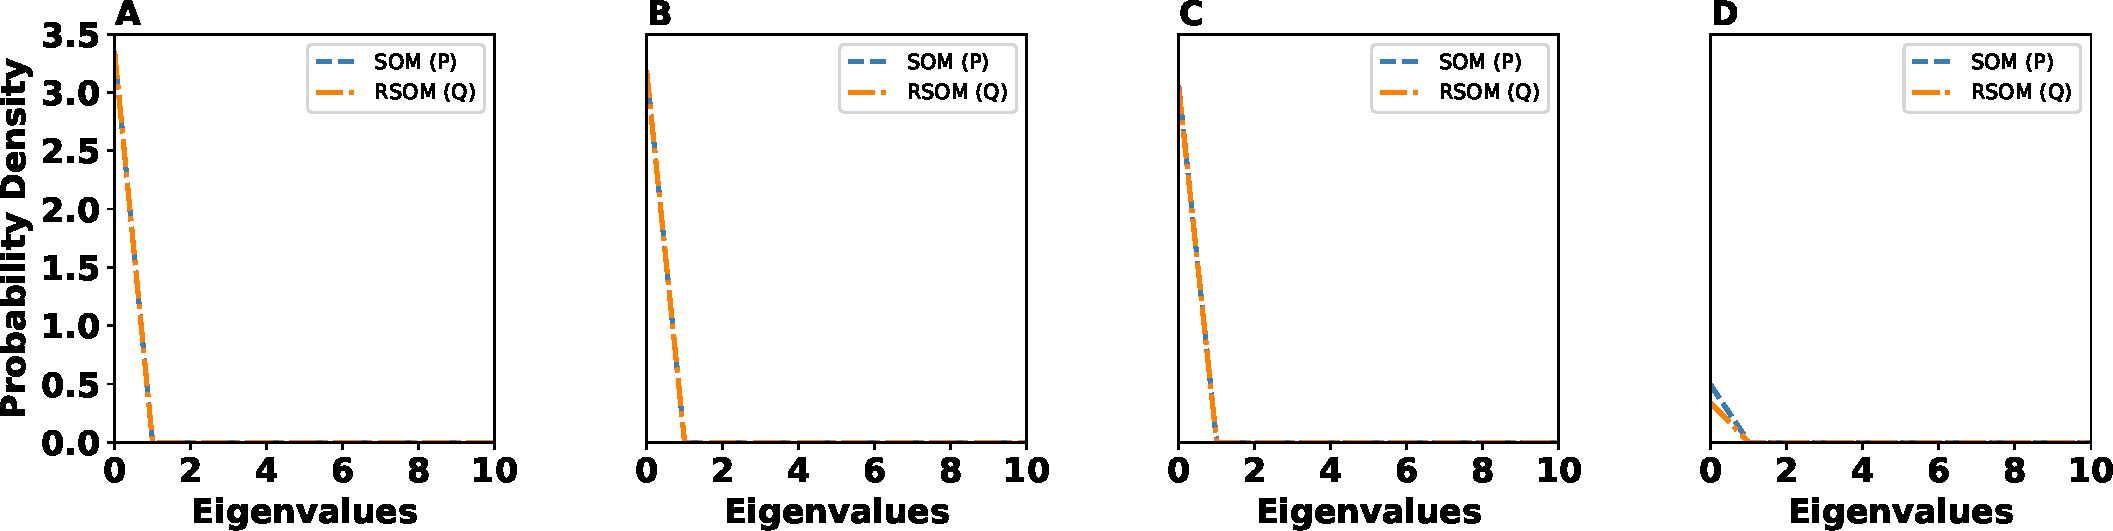
\includegraphics[width=\columnwidth]{eig-distributions-new.pdf}
  %
  \caption{Eigenvalues distribution for \textbf{A} 2D Ring dataset \textbf{B} 2D uniform dataset with holes \textbf{C} 3D uniform dataset and \textbf{D} MNIST Dataset
  }%
  \label{fig:eigenvalues}
 \end{figure}
